%%%%%%%%%%%%%%%%%%%%%%%%%%%%%%%%%%%%%%%%%%%%%%%%%%%%%%%%%%%%%%%%%%%%%%%%%%%%%%%
% Projeto para concurso público de Pesquisador Adjunto I em Sismologia.
%
% Formatação inspirada em:
% * https://github.com/leouieda/memorial2023
% * https://github.com/birocoles/memos

%%%%%%%%%%%%%%%%%%%%%%%%%%%%%%%%%%%%%%%%%%%%%%%%%%%%%%%%%%%%%%%%%%%%%%%%%%%%%%%

%%%%%%%%%%%%%%%%%%%%%%%%%%%%%%%%%%%%%%%%%%%%%%%%%%%%%%%%%%%%%%%%%%%%%%%%%%%%%%%
% Set a class and import packages
\documentclass[10pt,a4paper,oneside]{book}

% Variables
\newcommand{\Year}{2024}
\newcommand{\Author}{Diogo Luiz de Oliveira Coelho}
\newcommand{\Title}{Projeto de \Author{} para concurso público - Pesquisador Adjunto I em Sismologia - ON/MCTI}
\newcommand{\Email}{diogoloc@on.br}
\newcommand{\EmailPersonal}{locdiogo@gmail.com}
\newcommand{\ORCID}{0000-0001-5426-0455}
\newcommand{\ResearchGate}{https://www.researchgate.net/profile/Diogo-De-Oliveira-Coelho}
\newcommand{\Lattes}{4330106475199471}

% Import packages
\usepackage[utf8]{inputenc}
\usepackage[T1]{fontenc}
\usepackage[brazil]{babel}
\usepackage{geometry}
\usepackage{graphicx}
\usepackage{amssymb}
\usepackage{amsmath}
\usepackage{mathpazo}
\usepackage{hyperref}
% create fancy headers
\usepackage{fancyhdr}
% commands for managing dates and its formats
\usepackage{datetime2}
% improved urls with proper hyphenation
\usepackage{xurl}
% Control over enumerate and itemize
\usepackage{enumitem}
% Tweak the look of captions
\usepackage{caption}
% To control the style of section titles
\usepackage{titlesec}
% Add the bibliography to the table of contents
\usepackage[nottoc,chapter]{tocbibind}
\usepackage[round,authoryear,sort]{natbib}
% show dois as links on references
\usepackage{doi}
% Icon and fonts (requires using xelatex or luatex)
\usepackage{fontawesome5}
\usepackage{academicons}
\usepackage{fontspec}
\usepackage[mono]{notomath}
% To make everything neater
\usepackage{microtype}
% To make fancy text boxes
\usepackage{xcolor}
\usepackage[framemethod=default]{mdframed}
% For fancy and multipage tables
\usepackage{tabularx}
\usepackage{ltablex}
% To define custom environments
\usepackage{environ}
\usepackage{setspace}
% Reference sections by name
\usepackage{nameref}
% Better handling of footnotes inside summary boxes
\usepackage{footmisc}

%to rotate the page
\usepackage{pdflscape}

%To plot piechart
\usepackage{bera}
\usepackage{pstricks-add}
\usepackage{pgf-pie}

%%%%%%%%%%%%%%%%%%%%%%%%%%%%%%%%%%%%%%%%%%%%%%%%%%%%%%%%%%%%%%%%%%%%%%%%%%%%%%%

%%%%%%%%%%%%%%%%%%%%%%%%%%%%%%%%%%%%%%%%%%%%%%%%%%%%%%%%%%%%%%%%%%%%%%%%%%%%%%%
% Configuration of the document

\geometry{%
  left=30mm,
  right=30mm,
  top=20mm,
  bottom=15mm,
  headsep=5mm,
  headheight=5mm,
  footskip=10mm,
  includehead=true,
  includefoot=true
}

% Increase the line spacing
\SetSinglespace{1.2}
\onehalfspacing

% Remove spacing between enumerate/itemize items
\setlist{nosep}

% Padding between the first figure and the chapter title
\newcommand{\HeroFigPad}{\vspace{-1cm}}

% Padding before the software logo figures
\newcommand{\SoftwareFigPad}{\vspace{-0.3cm}}

% Add a link to a DOI
\newcommand{\DOI}[1]{\url{https://doi.org/#1}}

% Add a link to a GitHub repository
\newcommand{\GitHub}[1]{\faGithub{} Código: \url{https://github.com/#1}}

% Add a link to a YouTube video
\newcommand{\YouTube}[1]{\faYoutube{} Vídeo: \url{https://youtu.be/#1}}

% Add a link to a supplementary data
\newcommand{\Data}[1]{\faChartBar{} Dados: \url{https://doi.org/#1}}

% Add a link to a preprint
\newcommand{\Preprint}[1]{\faLockOpen{} Preprint: \url{https://doi.org/#1}}

% Make a Unicode bullet symbol
\newcommand{\Bullet}{•\enspace}

% Define custom colors
\definecolor{lu_gray}{gray}{0.98}
\definecolor{lu_darkgray}{gray}{0.3}
\definecolor{gold(metallic)}{rgb}{0.83, 0.69, 0.22}
\definecolor{cornsilk}{rgb}{1.0, 0.97, 0.86}
\definecolor{lu_blue}{RGB}{32, 96, 194}
\definecolor{lu_lightblue}{RGB}{238, 245, 250}
\definecolor{timberwolf}{rgb}{0.86, 0.84, 0.82}
\definecolor{battleshipgrey}{rgb}{0.52, 0.52, 0.51}

% Customize how Chapter headings are displayed
\titleformat{\chapter}[display]{\normalfont}{\large Capítulo \thechapter}{0pt}{\huge}[\titlerule]
\titlespacing*{\chapter}{0pt}{-40pt}{40pt}

% Set the spacing between bibliography entries (requires natbib)
\setlength{\bibsep}{0pt}

% Configure captions
\captionsetup{labelfont=bf,font={small,color=lu_darkgray},skip=0pt}

% Define a fancy text box
\mdfdefinestyle{summarybox}{%
  leftline=true,
  rightline=false,
  topline=false,
  bottomline=false,
  linewidth=4pt,
  linecolor=gold(metallic),
  frametitlefont=\bfseries\color{black}\small,
  frametitlebackgroundcolor=cornsilk,
  frametitleaboveskip=7pt,
  frametitlebelowskip=7pt,
  frametitlerule=true,
  frametitlerulewidth=1pt,
  backgroundcolor=lu_gray,
  innertopmargin=7pt,
  innerbottommargin=10pt,
  innerleftmargin=15pt,
  innerrightmargin=15pt,
  skipbelow=5pt,
  skipabove=0pt,
}
\newmdenv[style=summarybox]{summarybox}
\mdfdefinestyle{subsummarybox}{%
  leftline=true,
  rightline=false,
  topline=false,
  bottomline=false,
  linewidth=4pt,
  linecolor=battleshipgrey,
  frametitlefont=\bfseries\color{black}\small,
  frametitlebackgroundcolor=timberwolf,
  frametitleaboveskip=7pt,
  frametitlebelowskip=7pt,
  frametitlerule=true,
  frametitlerulewidth=1pt,
  backgroundcolor=lu_gray,
  innertopmargin=7pt,
  innerbottommargin=10pt,
  innerleftmargin=15pt,
  innerrightmargin=15pt,
  skipbelow=5pt,
  skipabove=0pt,
}
\newmdenv[style=subsummarybox]{subsummarybox}

% Define something like an fa-ul and a date list
\NewEnviron{fa-ul}{%
  \vspace{-0.4cm}
  \small
  \renewcommand{\arraystretch}{1.25}
  \begin{tabularx}{\linewidth}{@{}p{0.05\linewidth}@{}@{}p{0.95\linewidth}@{}}
    \BODY
  \end{tabularx}%
}
\NewEnviron{datelist}{%
  \vspace{-0.4cm}
  \small
  \renewcommand{\arraystretch}{1.25}
  \begin{tabularx}{\linewidth}{@{}p{0.15\linewidth}@{}@{}p{0.85\linewidth}@{}}
    \BODY
  \end{tabularx}%
}
\NewEnviron{paperlist}{%
  \vspace{-0.4cm}
  \small
  \renewcommand{\arraystretch}{1.25}
  \begin{tabularx}{\linewidth}{@{}p{0.08\linewidth}@{}@{}p{0.92\linewidth}@{}}
    \BODY
  \end{tabularx}%
}
\NewEnviron{courselist}{%
  \vspace{-0.4cm}
  \small
  \renewcommand{\arraystretch}{1.25}
  \begin{tabularx}{\linewidth}{@{}p{0.15\linewidth}@{}@{}p{0.85\linewidth}@{}}
    \BODY
  \end{tabularx}
}

% Define a fancy enumerate that has a title
\NewEnviron{fancyenum}[2]{%
  \vspace{0.25cm}
  \noindent#1\quad\textbf{#2}:
  \vspace{0.25cm}
  \begin{enumerate}
    \BODY
  \end{enumerate}
}

% Configure hyperref and add PDF metadata
\hypersetup{
    colorlinks,
    allcolors=lu_blue,
    pdftitle={\Title},
    pdfauthor={\Author},
    pdftex,
    breaklinks=true,
}

% make urls use the same font as every other text
\urlstyle{same}

% Prevent footnotes from being broken into multiple pages
\interfootnotelinepenalty=10000

% Configure headers and footers
\fancyhf{}
\lhead{\fontsize{9pt}{0}\selectfont\itshape \nouppercase\leftmark}
\chead{}
\rhead{\fontsize{9pt}{0}\selectfont \thepage}
\cfoot{}
\renewcommand{\headrulewidth}{0.3pt}
%%%%%%%%%%%%%%%%%%%%%%%%%%%%%%%%%%%%%%%%%%%%%%%%%%%%%%%%%%%%%%%%%%%%%%%%%%%%%%%

%%%%%%%%%%%%%%%%%%%%%%%%%%%%%%%%%%%%%%%%%%%%%%%%%%%%%%%%%%%%%%%%%%%%%%%%%%%%%%%
\begin{document}

\pagestyle{plain}
\frontmatter

\begin{titlepage}
  \begin{center}
    
\includegraphics[height=0.5cm]{images/logo_seismo.png}
    \vspace{1cm}

    CONCURSO PÚBLICO
    
    PESQUISADOR ADJUNTO I EM SISMOLOGIA
    
    OBSERVATÓRIO NACIONAL

    \vspace{5cm}

    \textbf{\LARGE Projeto}
    \vspace{1cm}

    \textbf{\LARGE \MakeUppercase{\Author{}}}
    \vspace{5cm}

    {\small
	Apresentado para concurso público de provas e títulos para cargo de

	Pesquisador Adjunto I em Sismologia do Observatório Nacional.
      \vspace{1cm}

	EDITAL N$^{\circ}$   1, DE 9 DE OUTUBRO DE 2023
    }
    \vfill

    \Year{}
  \end{center}
\end{titlepage}

%==============================================================================
\chapter*{Resumo}

Ao longo da minha trajetória acadêmica, obtive sucesso ao concluir o bacharelado em \href{https://geologia.ufes.br/}{Geologia} pela Universidade Federal do Espírito Santo, o mestrado em \href{https://www.gov.br/observatorio/pt-br/assuntos/programas-academicos/pos-graduacao-em-geofisica/pos-graduacao-em-geofisica}{Geofísica} pelo Observatório Nacional e o doutorado em \href{https://posgraduacao.ufrn.br/325}{Geodinâmica e Geofísica} pela Universidade Federal do Rio Grande do Norte. Durante minha formação acadêmica, tive a oportunidade de passar por três instituições de ensino superior ligadas ao Ministério da Educação (MEC), uma unidade de pesquisa vinculada ao Ministério da Ciência, Tecnologia e Inovações (MCTI), além de realizar estágio de nível superior na Petrobras, uma empresa estatal do setor de energia. Nessa caminhada acadêmica, tive a oportunidade enriquecedora de vivenciar de perto instituições públicas em quatro estados distintos do país. Essa diversidade geográfica proporcionou-me um aprendizado valioso e o aprimoramento da minha atuação na academia. Desde minha entrada no Observatório Nacional, ministrei a disciplina de \href{https://www.gov.br/observatorio/pt-br/assuntos/programas-academicos/pos-graduacao-em-geofisica/grade-curricular}{Introdução à Sismologia} em nível de pós-graduação, cursos de curta duração para graduandos em outras instituições e orientei alunos de iniciação científica. No âmbito da divulgação e popularização da ciência, redigi diversas notas técnicas tanto para a instituição quanto para veículos de imprensa. Além disso, participei de mais de 35 eventos relacionados a popularização e divulgação da ciência, dentre feiras de tecnologia, entrevistas para diversos canais da imprensa, podcast, revisão de textos e notas técnicas explorando temas variados da sismologia, incluindo sua relação com desastres naturais, bem como curiosidades gerais da população sobre a atuação de um pesquisador em geofísica. Desde o mestrado, tenho atuado na área de Sismologia e Tectônica da Crosta. Já no doutorado iniciei, de forma sistemática, o processo de desenvolvimento de diversos códigos em \href{https://www.python.org/}{python} para a sismologia, incluindo \href{https://github.com/dIOGOLOC/codes_escritos/tree/master/mantle_transition_zone_migration_obspy_Pds}{Receiver Migration}, \href{https://zooxantelapy.readthedocs.io/en/latest/}{Zooxantelapy} e \href{https://github.com/dIOGOLOC/marefone/wiki}{Marefone}. O primeiro pacote está relacionado a estruturação do manto terrestre e os dois últimos à dados oriundos de redes subaquáticas, às quais iniciei o tratamento e processamento de dados em 2020. Este memorial apresenta de forma resumida minha formação e atuação acadêmica, incluindo algumas considerações sobre os fatores que influenciaram na minha trajetória e os principais ensinamentos adquiridos ao longo dessa jornada que me ajudaram fazer pequenos ajustes na rota até aqui.

\begin{landscape}
% Conteúdo da página em modo paisagem
\begin{figure}[tb]
  \begin{center}
    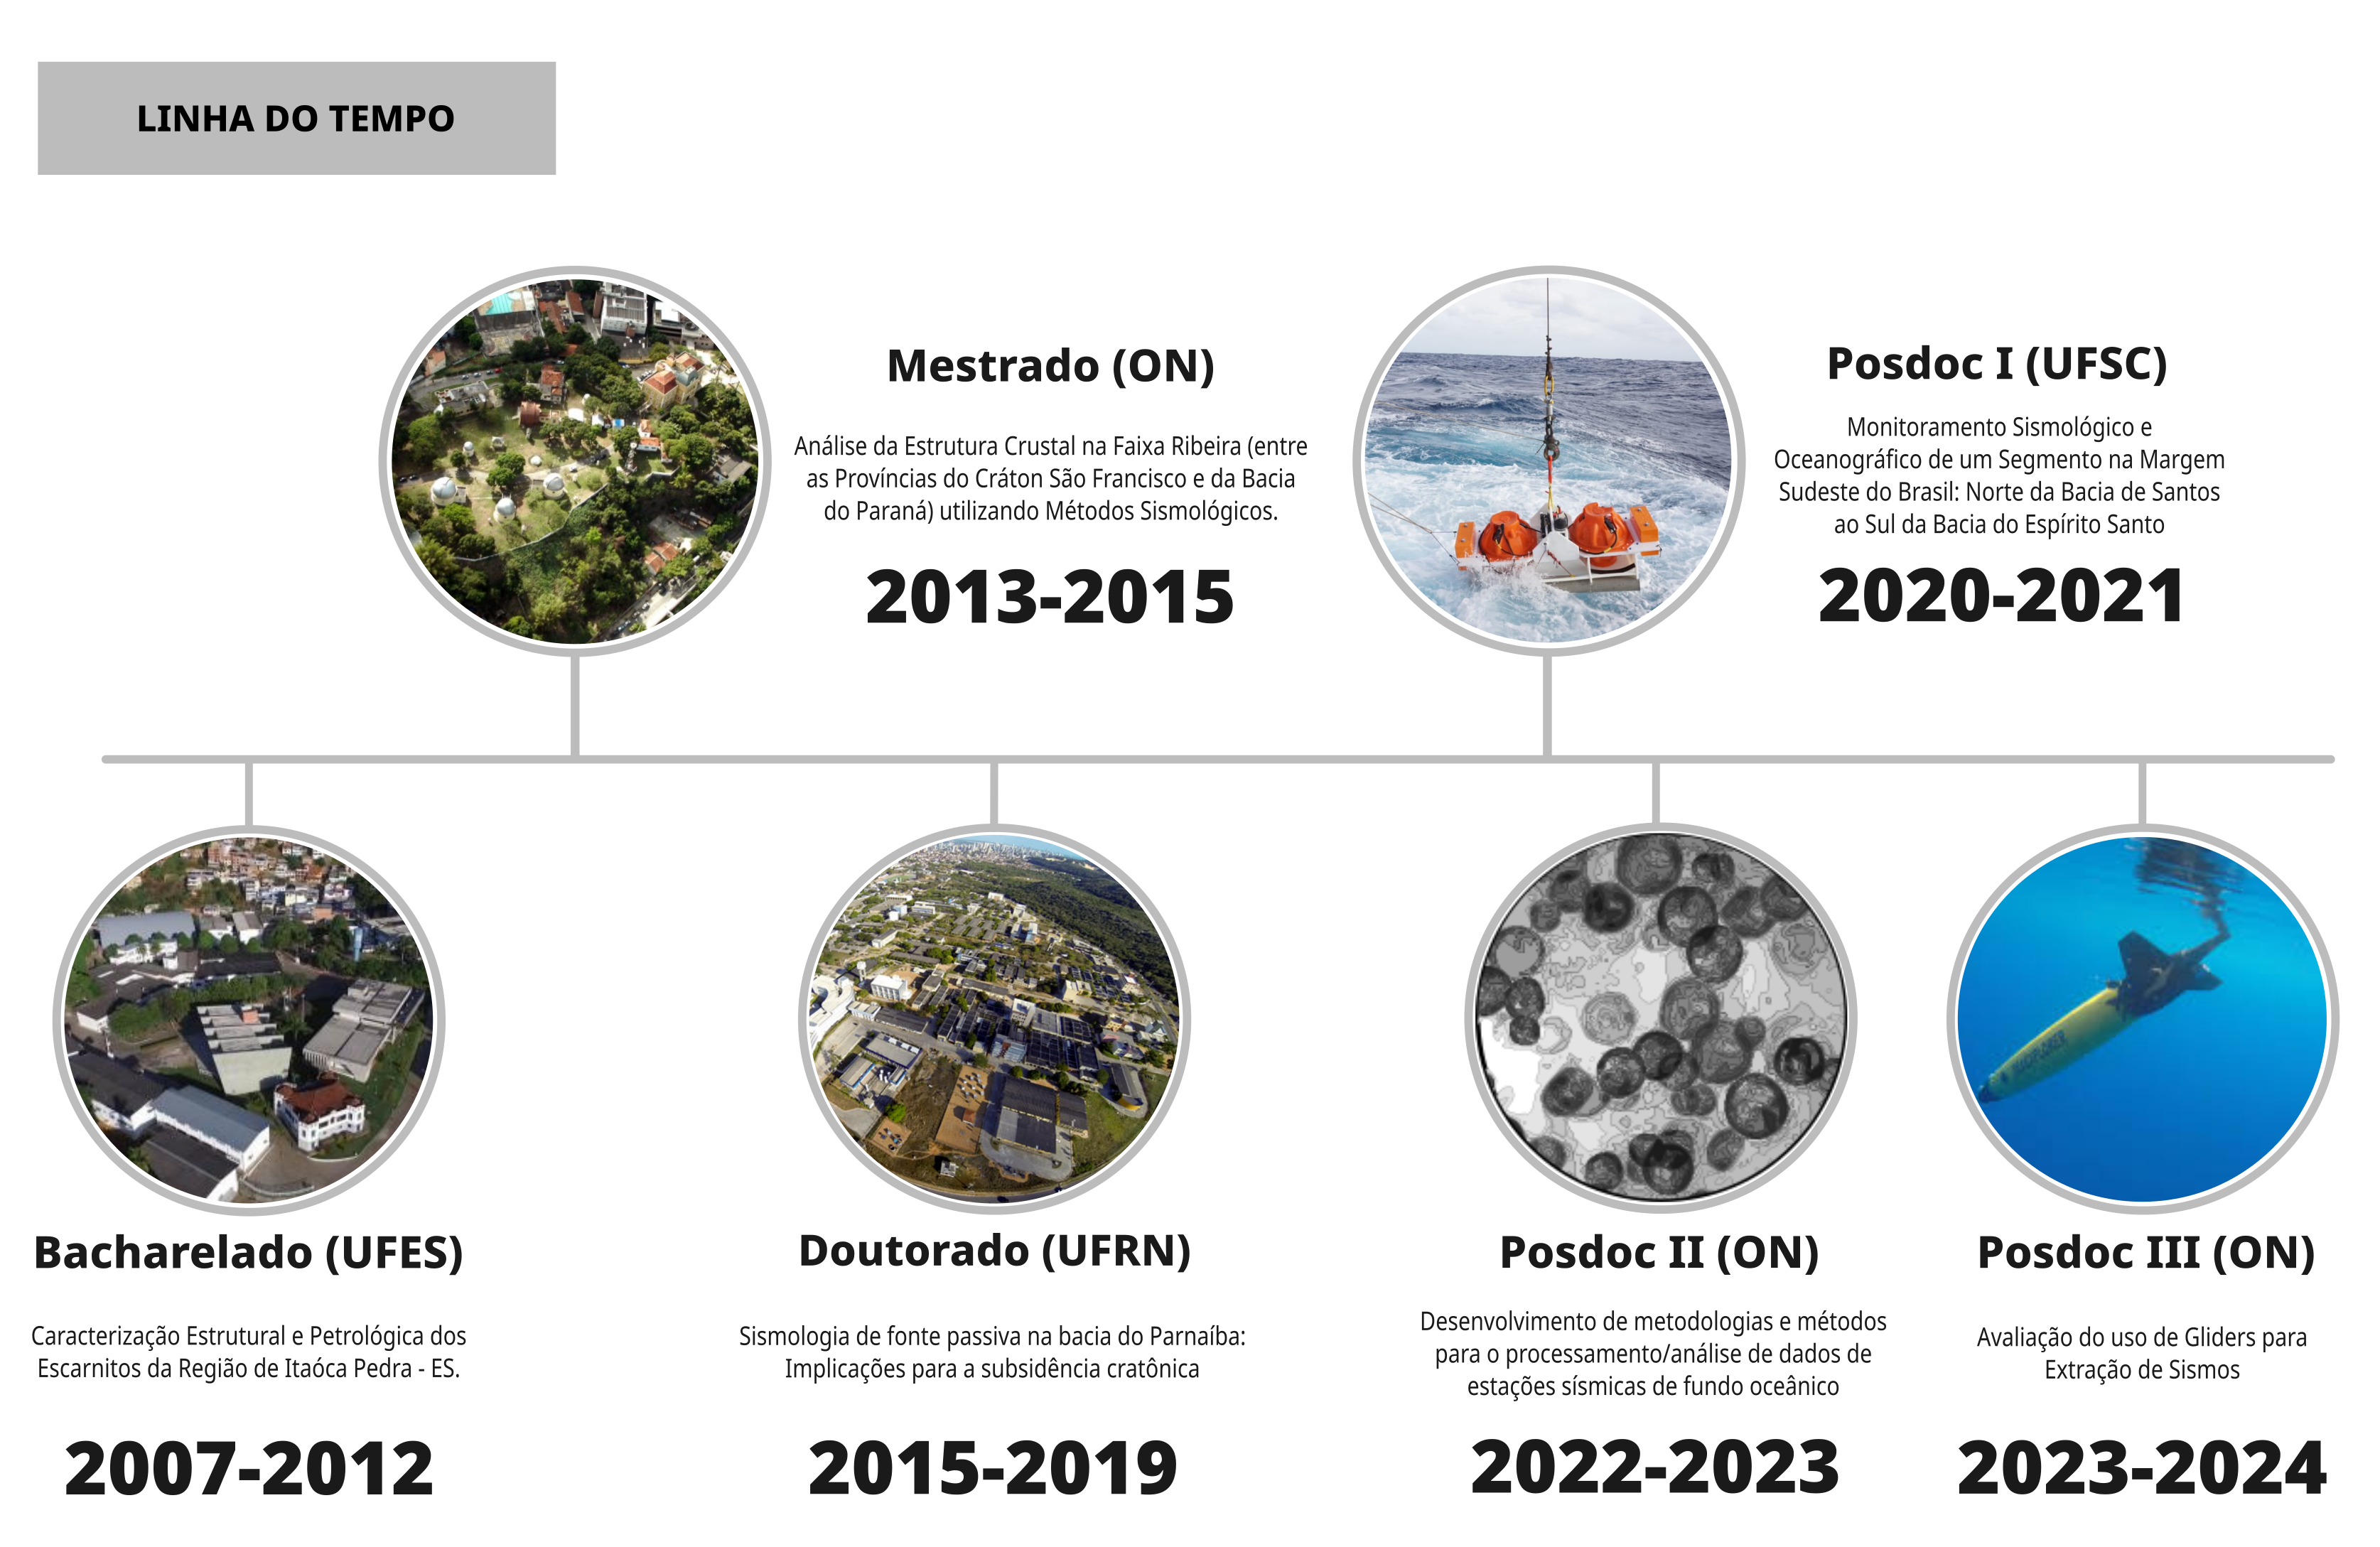
\includegraphics[width=\pagewidth]{images/linha_do_tempo.png}
  \end{center}
  \caption*{
    Resumo da minha trajetória acadêmica, desde a entrada na graduação em Geologia na Universidade Federal do Espírito Santo em 2007 até meu terceiro estágio pós-doutoral no Observatório Nacional no ano de 2024.
    }
\end{figure}
\end{landscape}
%==============================================================================
\tableofcontents

\mainmatter
\pagestyle{fancy}

%==============================================================================
\chapter{Apresentação}

\begin{figure}[h]
  \HeroFigPad
  \begin{center}
    
\includegraphics[width=\textwidth]{images/inicio.png}
  \end{center}
  \caption{
    Visitando em 2023 o estádio de \href{https://vasco.com.br/sao-januario/}{São Januário}, a colina histórica. Por estar localizada a menos de 1 km do Observatório Nacional, a sede do Vasco da Gama foi um dos principais fatores que me motivaram a entrar no programa de pós-graduação do Observatório Nacional.
  }
  \label{fig_riacho}
\end{figure}

Os textos devem ser apresentados em papel branco, formato A4, impressos somente na frente do papel, na cor preta, podendo utilizar outras cores somente para as ilustrações. 

O projeto gráfico é de responsabilidade do autor da pesquisa.

A fonte recomendada para a digitação é tamanho 12 para todo o texto, sendo que as citações com mais de três linhas devem ser digitado com tamanho menor e uniforme, além de ter o recuo de 4cm da margem esquerda.

Todo o texto deve ser digitado com o espaço entrelinhas de 1,5.

Os títulos das subseções devem ser separados do texto que os precede ou os sucede por dois espaços 1,5 (dois ENTER total = 3cm)

Os títulos sem indicativo numérico ( sumário, referencias, apêndices e anexos) devem ser centralizados.

As citações devem ser de acordo com as normas da ABNT, NBR10520, ago. 2002

\bigskip

\begin{summarybox}[frametitle=\faIcon{address-card}{}\quad Informações para contato]
  \begin{fa-ul}
    \faIcon{at} & email profissional: \href{mailto:\Email}{\Email} \\
    \faIcon{at} & email pessoal: \href{mailto:\EmailPersonal}{\EmailPersonal} \\
    \aiOrcid & ORCID: \href{https://orcid.org/\ORCID}{\ORCID} \\
    \aiResearchGate & ResearchGate: \href{\ResearchGate}{\ResearchGate} \\
    \aiLattes & Currículo Lattes: \url{https://lattes.cnpq.br/\Lattes} \\
    \faIcon{github} & Github: \url{https://github.com/diogoloc}
  \end{fa-ul}
\end{summarybox}

O Projeto de Pesquisa deve ser um roteiro para a elaboração de pesquisa em uma determinada área, que possibilita a produção do conhecimento e sua sistematização sobre o tema específico a ser abordando. O tema abordado deve constituir-se no objeto de estudo da pesquisa. A indicação do tema da pesquisa é o primeiro passo da elaboração do projeto.

O tema deve ser exposto de forma clara, apenas indicando o objeto a ser estudado. Para realizar o trabalho de investigação científica o pesquisador deverá definir e explicitar o tema ou objeto de análise de forma clara e direta. A delimitação do foco da pesquisa implica em situar o tema espacial (delimitação geográfica) e temporalmente (período proposto para a pesquisa), de acordo com o contexto geral da sua área de trabalho, assim como deve apresentar, já nesse momento, uma indicação do problema que será discutido acerca do tema.

O Projeto de pesquisa deve ser escrito de forma tal que pessoas não especialistas no tema, tais como as equipes das agências financiadoras ou organismos de política de pesquisa possam compreender os argumentos apresentados. Se for necessário utilizar termos muito especializados, estes devem ser definidos. Evitar uma linguagem pesada que dificulte a compreensão das idéias desenvolvidas pelo proponente.

Nesse mesmo sentido, tomar em consideração que o especialista a quem será encaminhado o projeto, deve ler muitos outros projetos. Se a redação é longa, complexa, desordenada, pouco clara, pedante e com erros ortográficos ou gramaticais, o especialista poderá até abandonar a leitura.

- Uma redação sintética, bem feita, é sinal de que o autor tem idéias bem claras e precisas do que pretende fazer. As probabilidades do projeto ser aprovado aumentarão.

%==============================================================================
\chapter{Estrutura do Projeto}
\label{cap_formacao}

\begin{figure}[h]
  \HeroFigPad
  \begin{center}
    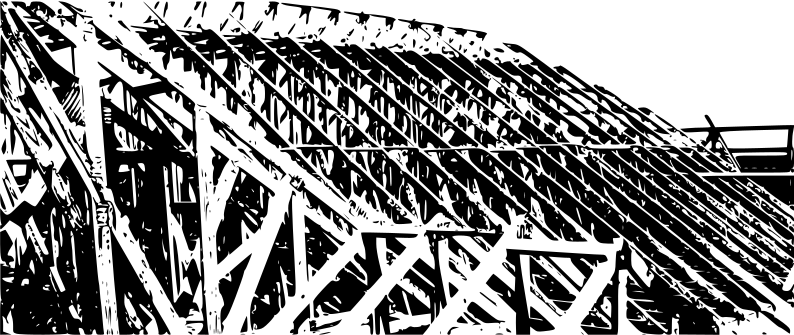
\includegraphics[width=\textwidth]{images/estrutura.png}
  \end{center}
  \caption{
    Visão da estrutura de um telhado (\href{https://cdn.b12.io/client_media/Mb9jai90/84e3b0f8-4fe0-11e9-a928-0242ac110003-jpg-regular_image.jpeg}{Fonte}).
  }
 \label{fig_formacao}
\end{figure}

\begin{summarybox}[frametitle=\faAward{}\quad Panorama sobre a estrutura do projeto]
  \begin{datelist}
    2007--2012 & Bacharelado em Geologia -- Universidade Federal do Espírito Santo \\
    2013--2015 & Mestrado em Geofísica -- Observatório Nacional \\
    2015--2019 & Doutorado em Geodinâmica e Geofísica -- Universidade Federal do Rio Grande do Norte
  \end{datelist}
\end{summarybox}

Este capítulo relata a minha trajetória acadêmica, da Graduação ao Doutorado, explorando alguns detalhes que foram cruciais na minha carreira e nos ajustes feitos durante o percurso.

\section{IDENTIFICAÇÃO}
\label{sec_ufrn}

\begin{subsummarybox}[frametitle=\faGraduationCap\quad Bacharelado em Geologia]
  \begin{fa-ul}
    \faFortAwesome & \textbf{Local:} Universidade Federal do Espírito Santo (Alegre-ES)\\
    \faClock & \textbf{Período:} Agosto 2007 -- Setembro 2012 \\
    \faUserTie & \textbf{Orientador:} Roberto Sacks de Campos\\
    \faChalkboardTeacher & \textbf{Tema:} Caracterização Estrutural e Petrológica dos Escarnitos da Região de Itaóca Pedra - ES.
  \end{fa-ul}
\end{subsummarybox}

IDENTIFICAÇÃO (caso seja necessário)

Área/Linha de Pesquisa:

Grupo de Pesquisa:

Departamento:

Campus Universitário:

Faculdade/Instituto:

Período de Execução:

Titulo: identificados na capa e na folha de rosto

Introdução:

Justificativa:

Objetivo: (Objetivos Gerais, Objetivos Específicos)

Fundamentação ou Referencial Teórico:

Metodologia (Materiais e Métodos, Hipóteses ou Questões Problemas)

Cronograma

Resultados Esperados:

Referencias

Apêndices

Anexos

MODELO DE CAPA: disponível no arquivo em PDF

MODELO DA FOLHA DE ROSTO: Disponível no arquivo em PDF

MODELO DO SUMÁRIO

SUMÁRIO
(Confira a ordem do conteúdo. A configuração correta está disponível no arquivo em PDF)


1 INTRODUÇÃO 
2 JUSTIFICATIVA 
3 OBJETIVOS 
4 FUNDAMENTAÇÃO TEÓRICA 
5 METODOLOGIA 
6 CRONOGRAMA 
7 RESULTADOS
REFERÊNCIAS
APÊNDICES 
ANEXOS


\subsection{O que é um projeto de pesquisa}
\label{sec_geo_basico}


O projeto é um documento através do qual se articula e se organiza uma proposta de pesquisa
e que se elabora, conforme DESLANDES (1996), orientado pelos seguintes aspectos:
a) Definição de um conjunto de recortes na realidade social.
b) Cartografia das escolhas para abordar a realidade, ou seja,
• O que pesquisar;
• Por que pesquisar;
• Como pesquisar.

\subsection{Finalidades do projeto}
\label{sec_geo_especifico}

As finalidades do projeto de pesquisa, na perspectiva proposta por DESLANDES (1996), são as seguintes:
a) Mapear o caminho a ser seguido durante a investigação; 
b) Orientar o pesquisador durante o percurso de investigação;
c) Comunicar os propósitos da pesquisa para a comunidade científica. 

\subsection{Elementos constitutivos do projeto}
\label{sec_bolsa_hidro}

\begin{summarybox}[frametitle=\faProjectDiagram{}\quad Resumo do projeto]
  \begin{datelist}
    \faFile* & Levantamento Hidrogeológico do Estado do Espírito Santo \\
    \faHammer & Universidade Federal do Espírito Santo e Universidade Federal do Ceará \\
    \faCalendar*[regular] & 24 meses \\
    \faMapMarked* & 37 municípios dos Espírito Santo \\
    \faUserTie & Paulo de Tarso Ferro de Oliveira Fortes \\
    \faWallet & Petrobras \\
    \faMoneyBill*[regular] & R\$ 3.447.638,38
  \end{datelist}
\end{summarybox}

O projeto é composto por elementos teóricos e metodológicos, conforme se especifica no
quadro a seguir. 

\begin{itemize}
	\item Referenciais teóricos
	\begin{itemize}
		\item Tema, problema, hipótese, objetivo geral, objetivos específicos, justificativa. 
	\end{itemize}
	\item Referenciais metodológicos 
	\begin{itemize}
		\item Metodologia: amostragem, formas de coleta, de organização e de análise dos dados.
	\end{itemize}
	\item Elementos complementares 
	\begin{itemize}
		\item Bibliografia, Equipe, Produtos, Cronograma, Orçamento 
	\end{itemize}
\end{itemize}


\subsection{Constituição formal do projeto}
\label{sec_bolsa_petro}

\begin{summarybox}[frametitle=\faInfoCircle{}\quad Resumo do estágio]
  \begin{datelist}
    \faFile* & Estágio Supervisionado em Geologia \\
    \faCalendar*[regular] & 3 meses (Junho a Agosto) \\
    \faMapMarked* & E\&P-SERV/US-SUB/GM (Geologia Marinha/Macaé-RJ) \\
    \faUserTie & Marco Aurélio de Campos Merschmann \\
    \faWallet & Petrobras
  \end{datelist}
\end{summarybox}

O projeto final deve conter obrigatoriamente os seguintes itens:

• Introdução
Apresentação do tema e do problema;
• Justificativa
Texto no qual se articulam os argumentos, de forma a demonstrar a relevância do tema.
• Referencial teórico
Destina-se a apresentar as leituras e fundamentos teóricos que embasam a proposta da pesquisa
• Objetivos
 a) Objetivo geral – apresentam-se de forma global os objetivos pretendidos na pesquisa;
 b) Objetivos específicos – corresponde aos desdobramentos do objetivo geral, de forma a traduzir, em suas diferentes especificidades, o que se pretende alcançar.
• Metodologia
Descreve-se os caminhos metodológicos previstos e as técnicas a serem utilizadas.
• Bibliografia
Referencia-se o material utilizado para o projeto e/ou da pesquisa, de acordo com as Normas da ABNT.
• Cronograma 
Destina-se a traduzir as ações a serem realizadas, distribuindo-as no espaço de tempo disponível para
a realização do projeto. 


%==============================================================================

\chapter{Linhas de Pesquisa}
\label{cap_pesquisa}

\begin{figure}[h]
  \HeroFigPad
  \begin{center}
    
\includegraphics[width=\textwidth]{images/inicio.png}
  \end{center}
  \caption{
    Compilação de resultados obtidos em três linhas de pesquisa distintas. Esquerda: Sismograma e espectrograma do terremoto local de 4.2 de magnitude do dia 25/03/2020 às 11:30:00, registrado na componente vertical de um OBS. Centro: Análise do banco de dados acústicos de glider oceânico do dia 02/08/2019 entre às 05:58:30 e 06:08:30. Direita: Comparação entre dados Sintéticos e Reais para a  espessura da Zona de Transição do Manto abaixo da Bacia do Parnaíba.
  }
\end{figure}

Neste capítulo, apresento de forma resumida os focos de investigação explorados no desenvolvimento da minha carreira acadêmica. Esta trajetória é marcada pela evolução dos interesses de pesquisa e pela busca contínua por desafios e conhecimento. Inicialmente, fui influenciado por temas intrinsecamente ligados à Geologia, especialmente Geomorfologia e Tectônica. Tal escolha foi guiada não apenas devido a minha formação na área, mas também pela minha fascinação por processos geológicos que moldam a superfície do nosso planeta, assim como a atuação da dinâmica das placas litosféricas e movimentos mantélicos ao longo do tempo geológico. No entanto, ao longo do doutorado, a introdução da programação como uma ferramenta complementar expandiu o meu leque de atuação. Esse novo caminho permitiu um aprendizado mais prático dos métodos e da modelagem computacional, enriquecendo ainda mais minha atuação científica. No estágio pós-doutoral, optei por uma abordagem mais flexível em relação aos temas de pesquisa, incorporando o monitoramento sísmico e hidroacústico. Aproveitando as oportunidades disponíveis, efetuei mudanças significativas de direcionamento, refletidas na expansão das linhas de pesquisa nas quais estou atualmente engajado. 

\section{Estruturação da Crosta e do Manto Superior}

\begin{summarybox}[frametitle=\faProjectDiagram{}\quad Panorama da linha de pesquisa]
	\begin{datelist}
		\faFile* & \textbf{Número de projetos:} 4 \\
		\faBinoculars & \textbf{Equipamentos:} Sismômetros banda larga e período curto \\
		\faCalendar*[regular] & \textbf{Período:} 2013 - atual \\
		\faMapMarked* & \textbf{Regiões:} Faixa Ribeira, Bacia do Parnaíba, ilhas oceânicas e bacias costeiras. \\
	\end{datelist}
\end{summarybox}

\bigskip

Esta linha de pesquisa busca revelar a estruturação profunda da Terra através de uma gama de metodologias, dentre as quais temos: \href{https://doi.org/10.1029/JB084iB09p04749}{Função do Receptor}, \href{https://doi.org/10.1111/j.1365-246X.1990.tb04573.x}{Dispersão de Ondas de Superfície}, \href{https://doi.org/10.1046/j.1365-246x.2000.00217.x}{Inversão Conjunta}, \href{https://doi.org/10.1016/j.epsl.2013.08.025}{Migração das Funções do Receptor} e \href{https://doi.org/10.1111/j.1365-246X.2007.03374.x}{Tomografia de Ruído Sísmico}. Esta linha de pesquisa está intimamente ligada à minha trajetória acadêmica, uma vez que minha formação prévia em Geologia, combinada com os resultados obtidos pelos métodos sismológicos, contribuem para uma visão abrangente da composição e dinâmica da subsuperfície terrestre. A caracterização da estrutura profunda das bacias cratônicas, faixas móveis e cratons permitem a identificação de padrões de sedimentação, processos geodinâmicos associados e processos de formação de montanhas, falhas e outros elementos estruturais. Além disso, a investigação da estrutura do manto superior, principalmente da zona de transição, fornece informações cruciais sobre a composição, temperatura e movimentos do manto superior, contribuindo para o entendimento dos processos de convecção e circulação mantélica que impulsionam a dinâmica global do planeta.  

\begin{fancyenum}{\faFutbol}{Objetivos}
	\item Imagear as principais descontinuidades crustais e mantélicas;
	\item Caracterizar a estrutura crustal profunda das principais provincias geológicas do Brasil;
	\item Investigar a composição, temperatura e fluxos do manto superior;
	\item Desenvolver rotinas computacionais mais eficientes para estimar as profundidade e espessuras das camadas em subsuperfície.
\end{fancyenum}

\begin{fancyenum}{\faCogs}{Principais contribuições}
	\item Estimativas da espessura das principais camadas abaixo de bacias intracratônicas;
	\item Contribuições no entendimento dos processos profundos atuantes em bacias sedimentares intracratônicas no Brasil;
	\item Rotina computacional para o cálculo das Funções do Receptor de onda P inteiramente em python;
	\item Programa eficiente para realizar a migração pré-empilhamento das Funções do Receptor de onda P.
\end{fancyenum}

\section{Instrumentação e Controle de Qualidade de dados na Sismologia}
\label{sec_inst_qc}

\begin{summarybox}[frametitle=\faProjectDiagram{}\quad Panorama da linha de pesquisa]
	\begin{datelist}
		\faFile* & \textbf{Número de projetos:} 4 \\
		\faBinoculars & \textbf{Equipamentos:} Sismômetros banda barga, sismômetros de fundo oceânico, sismógrafos flutuantes e planadores subaquáticos \\
		\faCalendar*[regular] & \textbf{Período:} 2017 - atual \\
		\faMapMarked* & \textbf{Regiões:} Atividades e testes em laboratório \\
	\end{datelist}
\end{summarybox}

\bigskip

Esta linha de pesquisa concentra-se na instalação e otimização da instrumentação para coleta de dados, bem como em métodos para garantir a qualidade e integridade dos dados coletados. A estrutura e instrumentação adequada para cada contexto e o controle de qualidade são fundamentais para garantir a precisão e confiabilidade dos resultados, sendo essenciais para a interpretação dos processos geodinâmicos. Ao desenvolver e implementar novas metodologias de instalação e controle de qualidade, podemos melhorar significativamente nossa capacidade de detectar e interpretar eventos sísmicos, naturais ou antrópicos, contribuindo assim para uma compreensão mais profunda dos processos geodinâmicos. Bons exemplos de metodologias utilizadas nessa linha de pesquisa são orientadas pelo \href{https://services.iris.edu/mustang/}{MUSTANG}, um utilitário estatístico que utiliza métricas de qualidade de dados sísmicos e funções de densidade de probabilidade para analisar os dados sísmológicos do \href{https://www.earthscope.org/}{EarthScope} (consórcio dedicado a apoiar pesquisa e educação geofísica global transformadora). É nesse utilitário que eu me baseiei para confeccionar os programas para a análise de qualidade dos dados, como o \href{https://zooxantelapy.readthedocs.io/}{Zooxantelapy} e o \href{https://github.com/dIOGOLOC/codes_escritos/tree/master/LabSis_controle_de_qualidade}{LabSis: Controle de qualidade}.

\begin{fancyenum}{\faFutbol}{Objetivos}
  \item Desenvolver uma infraestrutura eficiente para a aquisição de dados sísmicos de alta qualidade;
  \item Estabelecer procedimentos de controle de qualidade robustos para garantir a integridade dos dados coletados;
  \item Fornecer recursos e ferramentas para análise e validação de dados sísmicos, principalmente para o banco de dados da Rede Sismográfica Brasileira.
\end{fancyenum}

\begin{fancyenum}{\faCogs}{Principais contribuições}
  \item Desenvolvimento de programas otimizados para o controle de qualidade completo do banco de dados;
  \item Implementação de sistemas automáticos de controle de qualidade de dados em redes de monitoramento sísmico;
  \item Contribuições para a padronização de práticas instalação de estações sismográficas em diversos contextos geológicos diferentes.
\end{fancyenum}

\section{Monitoramento Sísmico e Hidroacústico}
\label{sec_monitor_sis}

\begin{summarybox}[frametitle=\faProjectDiagram{}\quad Panorama da linha de pesquisa]
	\begin{datelist}
		\faFile* & \textbf{Número de projetos:} 3 \\
		\faBinoculars & \textbf{Equipamentos:} Sismômetros de fundo oceânico, sismógrafos flutuantes e planadores subaquáticos \\
		\faCalendar*[regular] & \textbf{Período:} 2020 - atual \\
		\faMapMarked* & \textbf{Regiões:} Bacia de Campos, Bancia de Santos e ilhas oceânicas. \\
	\end{datelist}
\end{summarybox}

\bigskip

Essa linha de pesquisa abrange métodos de monitoramento sismológico terrestre e marinho, visando compreender os eventos sísmicos e acústicos em diversas escalas temporais e espaciais. Isso inclui a detecção e análise de terremotos, atividade vulcânica, movimentos submarinos e até mesmo fenômenos relacionados à ação humana. Esse novo capítulo na minha jornada acadêmica reflete não apenas a evolução dos meus interesses de pesquisa, mas também o compromisso contínuo com a inovação e a busca por desafios científicos que contribuam para o avanço do conhecimento sismológico para a sociedade como um todo.

\begin{fancyenum}{\faFutbol}{Objetivos}
  \item Aplicação de métodos avançados eficientes de monitoramento sísmico e hidroacústico;
  \item Investigar a relação entre atividades sísmicas e fenômenos geodinâmicos;
  \item Classificação de eventos sísmicos em todo território nacional, principalmente em ambiente submarino.
\end{fancyenum}

\begin{fancyenum}{\faCogs}{Principais contribuições}
  \item Desenvolvimento de algoritmos para identificação de eventos sísmicos e acústicos, naturais e antrópicos;
  \item Implementação de um sistema de monitoramento sísmico/hidroacústico em ambiente submarino;
  \item Contribuições para a compreensão dos efeitos de atividades humanas nos padrões sísmicos e acústicos da margem Sudeste do Brasil.
\end{fancyenum}

% ==============================================================================

\chapter{Atividades de Ensino e Mentoria}
\label{cap_ensino}

\begin{figure}[h]
  \HeroFigPad
  \begin{center}
    
\includegraphics[width=\textwidth]{images/inicio.png}
  \end{center}
  \caption{
    Moisaico de imagens em atividades de ensino durante o estátio pós-doutoral no Observatório Nacional. Primeira: Ministrando um curso de python no Ciclo de Seminários do Programa de Pós-Graduação do Observatório Nacional. Segunda: Ministrando a palestra Sismologia: Adornando a Tectônica com Terremotos na Universidade Federal do Espírito Santo. Ministrando o minicurso na I Escola Itinerante da Geofísica do Observatório Nacional na Universidade Federal de Pernambuco.}
\end{figure}

\begin{summarybox}[frametitle=\faChalkboardTeacher{}\quad Resumo das atividades]
  \begin{fa-ul}
    \faStreetView & 2 orientações de alunos de iniciação científica \\
    \faBook & 1 disciplina de pós-graduação ministrada \\
    \faEdit & 3 cursos de curta duração ministrados \\
    \faNewspaper & Tópicos ensinados: Sismologia, Geologia, Tectônica, Programação (Python), Instrumentação sismológica e Geodinâmica.
  \end{fa-ul}
\end{summarybox}

As atividades de ensino e mentoria de alunos começaram formalmente apenas durante o estágio pós-doutoral. Essa falta de prática em atividades de ensino e orientação deve-se ao fato de que as bolsas de estudo concedidas para o mestrado e doutorado não exigem a realização de disciplinas ou estágios de docência. No entanto, é evidente o crescimento vertiginoso do conhecimento sismológico acumulado devido às orientações e aulas ministradas, além das oportunidades para aprender e desenvolver minhas habilidades interpessoais com outros acadêmicos. A forma de ensinar e orientar é fortemente influenciada pelas disciplinas estudadas durante a minha trajetória acadêmica, especialmente no que se refere à habilidade de selecionar e transmitir uma grande quantidade de conteúdo em um curto período de tempo. No entanto, a experiência familiar foi muito relevante neste tópico, pois a minha família é majoritariamente formada por professores da rede pública de ensino do Estado do Rio de Janeiro (\href{https://www.seeduc.rj.gov.br/}{SEEDUC}), e nas conversas informais eu aprendi diversas formas de interegir com uma turma diversa e oriunda realidades distintas. Ratificando o que foi dito anteriormente, todas as conversas com minhas tias que passaram décadas lecionando na Educação de Jovens e Adultos (\href{http://portal.mec.gov.br/index.php?option=com_docman&view=download&alias=13448-diretrizes-curiculares-nacionais-2013-pdf&Itemid=30192}{EJA}) me ajudaram a entender que a pesquisa na área das Geociências rompe com a simetria do ensino regular e impulsiona percursos individualizados, sendo a minha trajetória acadêmica um grande exemplo disso. Como a entrada no Programa de Pós-graduação em Geofísica é fomentada para uma gama de áreas do saber (e.g. graduados em Geofísica, Geologia, Física, Matemática ou áreas afins) é vital que o professor entenda a responsabilidade de estimular e viabilizar o acesso e a permanência do aluno na instituição, proporcionando oportunidades educacionais apropriadas de acordo com as características do aluno, seus interesses, condições de vida e de trabalho.

No desenvolvimento da minha prática docente, percebi que a computação é uma ferramenta poderosa para capacitar os alunos, não apenas na compreensão dos conceitos teóricos, mas também na aplicação prática desses conceitos. Através de atividades práticas, os alunos desenvolvem uma série de competências, incluindo análise de dados, resolução de problemas e pensamento crítico. Isso facilita a compreensão dos alunos e estimula sua curiosidade e interesse pelo assunto. Este capítulo oferece um breve relato das minhas atividades de ensino e orientação, destacando minha abordagem pedagógica e meu papel na ministração da disciplina de Introdução à Sismologia no Programa de Pós-graduação, onde busco promover um ambiente de aprendizado colaborativo e inclusivo, onde os alunos sintam-se capacitados a explorar e desenvolver seu potencial máximo.

\section{Orientações}
\label{sec_orientacao}

Minha primeira experiência como orientador é oriunda do Programa Institucional de Iniciação Científica e Tecnológica do ON (\href{https://www.gov.br/observatorio/pt-br/assuntos/programas-academicos/iniciacao-cientifica-e-tecnologica/apresentacao}{PICT/ON}), o qual é uma iniciativa da instituição como contrapartida ao programa de bolsas \href{http://portal-adm.cnpq.br/web/guest/pibic/}{PIBIC}, oferecido pelo Conselho Nacional de Desenvolvimento Científico e Tecnológico (\href{https://www.gov.br/cnpq/pt-br}{CNPq}). Esta iniciativa do ON ampliou o número de bolsas de Iniciação Científica e Tecnológica para alunos de graduação de diversas áreas. No entanto, um diferencial desse programa é permitir que alunos de outras Universidades, localizadas fora do Rio de Janeiro, possam desenvolver trabalhos junto a pesquisadores do ON. Dada a essa nova realidade, eu iniciei a orientação das alunas \href{http://lattes.cnpq.br/4746789434324199}{Ingrid Herzog} (\href{https://unipampa.edu.br/portal/}{Unipampa}) e \href{http://lattes.cnpq.br/6698175242371919}{Thereza Mayra de Souza Fialho} (\href{https://www5.usp.br/}{USP}) inteiramente online entre Setembro de 2022 e Março de 2024 (18 meses).

O projeto realizado pela Ingrid utilizou dados das estações sismográficas situadas no estado do Rio Grande do Sul a fim de desenvolver estudos sismológicos sobre a estrutura sob essas estações, procurando correlacionar os resultados com a história geotectônica local. Nesse contexto, o método da \href{http://eqseis.geosc.psu.edu/cammon/HTML/RftnDocs/rftn01.html#:~:text=Receiver\%20functions\%20are\%20time\%20series,Earth\%20structure\%20near\%20the\%20receiver}{função do receptor} tem sido usado com sucesso para estudar descontinuidades no limite crosta/manto ao redor do mundo. Os resultados desse projeto proporcionaram informações-chave para formular hipóteses, bem como confirmar alguns modelos propostos para as grandes estruturas crustais abaixo das estações e contribuiu para ajudar a determinar os processos evolutivos que ocorreram na área de estudo. Além disso, o projeto compilou um fluxo de processamento em python para o cálculo da espessura crustal, assim como propriedades complementares oriundas da metodologia da função do receptor que será disponibilizado para toda comunidade científica. A estudante realizou todo o processamento dos dados em algoritmos desenvolvidos em Python, utilizando os pacotes do \href{https://docs.obspy.org/}{ObsPy}, \href{https://seispy.xumijian.me/latest/}{Seispy} e \href{https://www.pygmt.org/latest/}{Pygmt}. Os resultados deste trabalhos foram satisfatórios e foram apresentados pela estudante como um resumo expandido no \href{https://sbgf.org.br/congresso/}{18 Congresso Internacional da Sociedade Brasileira de Geofísica e EXPOGEf} entre 16 e 19 de Outubro de 2023. O trabalho foi premiado pela Unipampa e a estudante foi contemplada com uma ajuda de custos para apresentar presencialmente seu poster no congresso. Além dessa premiação, o resumo expandido recebeu a indicação para publicação no \href{https://sbgf.org.br/revista/index.php/rbgf}{Brazilian Journal of Geophysics}. Contudo, no início de 2024 recebi a notícia que a Ingrid passou no processo seletivo para mestrado no \href{https://www.iag.usp.br/}{Instituto de Astronomia, Geofísica e Ciências Atmosféricas} da USP.

O projeto realizado pela Thereza teve como objetivo comparar as particularidades dos terremotos em Marte e inferir os principais agentes causadores da sismicidade no planeta vermelho. Utilizamos a biblioteca \href{https://docs.obspy.org/}{ObsPy} para leitura e tratamento dos dados do \href{https://www.insight.ethz.ch/seismicity/catalog/v13}{catálogo sísmico da missão InSight} e, para que eles fossem mais concisos, limitamos a observação de eventos para que tivéssemos não somente a magnitude, mas também a longitude e latitude para podermos comparar com as feições geológicas existentes e, se viável, traçar um paralelo com a Terra. O grande desafio do projeto foi aplicar métodos sismológicos em dados resultantes de apenas uma estação para estudar a distribuição dos sismos marcianos, que são fortemente ofuscados pela presença de tempestades de areia e de outros processos de superfície. O âmago deste projeto foi examinar os dados contínuos do \href{https://www.iris.edu/hq/sis/insight}{InSight SEIS} para buscar entender a sismicidade em Marte através da identificação dos principais eventos sísmicos catalogados e da distribuição da atividade sísmica na superfície de Marte. Esse trabalho abriu uma nova frente de pesquisa para mim, pois os meus trabalhos e linhas de pesquisa eram relacionados a Terra. Assim como aconteceu anteriormente, a Thereza também foi aprovada no processo seletivo de mestrado do \href{https://www.iag.usp.br/}{Instituto de Astronomia, Geofísica e Ciências Atmosféricas} da USP, portanto o projeto teve que ser finalizado.

\bigskip

\begin{summarybox}[frametitle=\faBookmark{}\quad Resumo dos trabalhos apresentados pelos alunos em congressos]
  \begin{fa-ul}
      \faBuilding & 18th International Congress of the Brazilian Geophysical Society \\
      \faBook & Thickness and crustal composition investigation in the Sul-rio-grandense Shield (SrgS) \\
      \faChild & HERZOG, I.; \textbf{COELHO, D. L. O.}; HISPAGNOL, N. R. ; LIMA, M. V. A. G. D.; GREGORY, T. R.\\
      \faCertificate & \href{https://sbgf.org.br/mysbgf/eventos/expanded_abstracts/18th_CISBGf/9778d5d219c5080b9a6a17bef029331cResumo_expandd_SBGF_INGL\%C3\%8AS.docx\%20(1).pdf}{Resumo Expandido}  \\
      \faCalendar & 2023 \\
  \end{fa-ul}
\end{summarybox}

Através dessas orientações, aprendi a orientar alunos sem experiência prévia em pesquisa através das etapas iniciais de um projeto e a adaptar o nível dos projetos propostos ao nível dos alunos. Foi gratificante receber a notícia de que os alunos progrediram em suas carreiras acadêmicas e que seus projetos alcançaram uma qualidade excelente, superando até mesmo as expectativas deles mesmos.

\section{Cursos de curta duração}
\label{sec_workshops}

Minha primeira experiência em outra instituição, divulgando e ensinando sob o regime de estágio pós-doutoral no Observatório Nacional, ocorreu por convite do professor \href{http://lattes.cnpq.br/4046823088402890}{Luiz Carlos de Carvalho Benyosef}, na Escola Itinerante de Geofísica do Observatório Nacional, realizada de 08 a 10 de agosto de 2023. Foi durante esse curso que percebi minha habilidade para lecionar e divulgar a pesquisa científica. Desde então, ministrei 3 cursos de curta duração e workshops em formato online e presencial. Esses cursos complementam o ensino convencional em Sismologia e Tectônica, oferecendo a chance de explorar diferentes tecnologias, métodos de ensino e temas menos convencionais. Além disso, também ministrei cursos relacionados a integração de Sismologia e Programação em python. O formato curto é adequado para uma introdução à conceitos básicos de programação ou para abordar um assunto específico (e.g., como ler e plotar gráficos de dados sismológicos, como manipular catálogos de eventos sísmicos ou como realizar tarefas simples em python). Mesmo com um orçamento limitado é possível desenvolver esses cursos, pois atualmente existem diversas plataformas de vídeo conferência.

\bigskip

\begin{subsummarybox}[frametitle=\faEdit{}\quad Seminários e workshops ministrados]
	\begin{paperlist}
		Ago/23  & Sismologia: existem terremotos no Brasil?
		\newline
		\faInfoCircle I Escola Itinerante de Geofísica do Observatório Nacional (presencial).
		\newline
		\faBuilding Universidade Federal de Pernambuco  (Recife-PE)
		\newline
		\faArchive{} \href{https://doi.org/10.6084/m9.figshare.25387180.v1}{Apresentação}
		\faBullhorn{} \href{https://www.ufpe.br/df/todos-os-informes/-/asset_publisher/znKKONCGSp59/content/a-primeira-escola-itinerante-de-geofisica-do-observatorio-nacional-ocorrera-na-ufpe-no-periodo-de-08-10-de-agosto-de-2023/441331}{Noticia}
		\\
		Set/23  & Desvendando Python: Uma Jornada de 40 Minutos.
		\newline
		\faInfoCircle Ciclo de seminários do PPGG/ON 2023 (presencial/online)
		\newline
		\faBuilding Observatório Nacional (Rio de Janeiro-RJ) 
		\newline
		\faGithub{} \href{https://github.com/dIOGOLOC/workshop_course_lecture/tree/6a0758f18303eecb6344a61fdbf874225da5e6be/ON_SET_2023}{Código}
		\faYoutube{} \href{https://youtu.be/LhRH2uYTWhc}{Vídeo}
		\\ 
		Out/23 & Sismologia e Python: Introdução prática ao processamento de dados sismológicos
		\newline
		\faInfoCircle XI Semana de Estudos Geológicos da Universidade Federal do Espírito Santo/IX Semana de Geologia do Espírito Santo (presencial)
		\newline
		\faBuilding Universidade Federal do Espírito Santo (Alegre-ES) 
		\newline
		\faArchive{} \href{https://doi.org/10.6084/m9.figshare.25387123.v1}{Apresentação}
		\faGithub{} \href{https://github.com/dIOGOLOC/workshop_course_lecture/tree/6a0758f18303eecb6344a61fdbf874225da5e6be/SEGEO_2023_UFES}{Código}
		\\
	\end{paperlist}
\end{subsummarybox}

\section{Disciplinas na pós-graduação}
\label{sec_ensino_grad}

Sou o responsável, juntamente com o professor \href{http://lattes.cnpq.br/8537150955145617}{Sergio Luiz Fontes}, pela disciplina \href{https://www.gov.br/observatorio/pt-br/assuntos/programas-academicos/pos-graduacao-em-geofisica/ementas/introducao-a-sismologia}{Introdução à Sismologia} onde ensino de maneira introdutória terremotos, estrutura da Terra, aquisição e processamento de dados sísmicos e instrumentação dentro nos diversos campos de atuação da \href{http://www.rsis.on.br/}{Rede Sismográfica do Sul e do Sudeste do Brasil (RSIS)}. Dada a complexidade da mecânica de terremotos e da geodinânima, aliados ao pouco tempo disponível para a disciplina (3 meses), o processo de avaliação que eu utilizado para mensurar o desempenho dos alunos está relacionado a confecção de três tipos de resumos (e.g. informativo, indicativo e crítico) sobre artigos científicos da área. A proposta desse processo de avaliação\footnote{Exemplos: avaliações \href{https://docs.google.com/forms/d/e/1FAIpQLSffa78ttrM_i5cWZmISGNz-lhwShi3Wzk7AUbWPgN6lhDuTNQ/viewform}{2} e \href{https://docs.google.com/forms/d/e/1FAIpQLSe8FIH4vSjn5QLT79BdG8eVRLti0le8i6yssInmQTX1iXNrYA/viewform}{3}} é ensinar aos alunos a elaboração de um resumo científico, tanto em português quanto em inglês, já que para a maioria deles, essa seria sua primeira experiência e contato com a escrita científica. Além disso, incorporei uma abordagem computacional introduzindo a manipulação de tabelas e dados de eventos sísmicos dentro do ambiente do \href{https://colab.google/}{google colab}, que é um serviço hospedado do \href{https://jupyter.org/}{Jupyter Notebook} que não requer configuração para ser usado e fornece acesso gratuito a recursos de computação. O Colab é especialmente adequado para aprendizado de máquina, ciência de dados e educação computacional básica. Como exemplos temos a \href{https://colab.research.google.com/drive/1c7Vc_s0A5GURJIab2vTS-LCW8fPlRaXt?usp=sharing}{aula de introdução ao Google colab} e a \href{https://colab.research.google.com/drive/17VaW0MkQxcxUjGaeowaVwyRORrijCXaV?usp=sharing}{aula de introdução ao Python}.

\bigskip

\begin{subsummarybox}[frametitle=\faGraduationCap{}\quad Disciplinas ministradas no Observatório Nacional]
  \begin{courselist}
    2022--2024 &
      SISMO - Introdução à Sismologia
      \newline
      \faInfoCircle \href{https://www.gov.br/observatorio/pt-br/assuntos/programas-academicos/pos-graduacao-em-geofisica/grade-curricular}{Grade Curricular}
      \newline
      \faInbox \href{https://www.gov.br/observatorio/pt-br/assuntos/programas-academicos/pos-graduacao-em-geofisica/ementas/introducao-a-sismologia}{Ementa}
  \end{courselist}
\end{subsummarybox}

Estou plenamente disponível e comprometido para ministrar essas novas disciplinas de Sismologia na pós-graduação. Com uma sólida experiência em pesquisa e análise de dados sísmicos, estou entusiasmado em oferecer aos alunos uma educação de alta qualidade e prepará-los para os desafios do mundo real. Estou confiante para trabalhar em colaboração com os alunos para promover uma compreensão profunda e abrangente da Sismologia e suas aplicações.

%==============================================================================


\chapter{Popularização da Ciência}
\label{cap_comunidade}

\bigskip

\begin{figure}[h]
  \HeroFigPad
  \begin{center}
    
\includegraphics[width=\textwidth]{images/inicio.png}
  \end{center}
  \caption{
    Moisaico mostrando as diversas frentes de atuação na divulgação e popularização da ciência durante o estágio pós-doutoral no Observatório Nacional. Esquerda: Participação com o Projeto Sismo-oceanográfico em 2022 no Rio Innovation Week. Centro: 3 fotos de entrevistas respondendo os questionamentos da sociedade em relação a sismicidade brasileira e global. Direita: Ministrando o mini-curso “Sismologia: existem terremotos no Brasil?” na Universidade Federal de Pernambuco.}
\end{figure}

Após ingressar no estágio pós-doutoral, cerca de um mês depois, o planeta iniciou um extenso período de \href{http://repositoriocovid19.unb.br/repositorio-produtos/desvelando-o-isolamento-social-no-cotidiano-vivido-na-pandemia-da-covid-19/}{isolamento social}. Foi nesse contexto que constatei uma crescente demanda social por informações científicas, além de identificar uma lacuna significativa em minha carreira nesse campo tão crucial na ciência contemporânea. Diante dessa necessidade evidente, iniciei minhas atividades voltadas para à divulgação e popularização da ciência junto à Divisão de Comunicação e Popularização da Ciência (\href{https://www.gov.br/observatorio/pt-br/assuntos/areas-de-atuacao/divulgacao-e-popularizacao-da-ciencia}{DICOP}), reconhecendo a importância de fornecer conhecimento acessível à sociedade. Este capítulo relata minhas atividades relacionadas a divulgação da ciência, como mostra a Figura \ref{fig_resumo_divulgacao}. Durante esse período, meu engajamento abrangeu a diversas demandas da DICOP em variadas plataformas de comunicação, abordando tanto o meio virtual, por meio de redes sociais e canais de imprensa online, quanto atividades presenciais, como feiras e eventos de divulgação científica e tecnológica, assim que as restrições permitiram.

\begin{figure}
	\centering
	\begin{tikzpicture}
	\pie{34.3/Entrevista escrita (13),
		21.0/Entrevista gravada (8),
		10.5/Revisão de texto (4),
		7.8/Evento Online (3), 
		7.8/Entrevista ao vivo (3),
		5.2/Evento presencial (2),
		5.2/Mini-curso (2),
		8/Outros (3)}
	\end{tikzpicture}
	\caption{Estatística das atividades de divulgação científicas realizadas entre 2020 e 2024.}
	\label{fig_resumo_divulgacao}
\end{figure}

Os números apresentados acima, assim como a lista \ref{lista_divulgacao}, fornecem uma visão detalhada dessa abordagem multifacetada na popularização da ciência e das atividades do Obseravtório Nacional ao longo do período que estive na instituição, um total de 38 atividades ao longo de 3 anos. Destaco que concedi dezenas de entrevistas, totalizando 24 (13 escritas, 8 gravadas e 3 ao vivo), contribuí revisando textos na temática da Sismologia e Geologia que foram publicados nas redes sociais do Obseravtório Nacional. Além disso, fiz parte da comitiva que participou do \href{https://www.gov.br/observatorio/pt-br/assuntos/areas-de-atuacao/divulgacao-e-popularizacao-da-ciencia/on-riw}{Rio Innovation Week}, o maior evento de tecnologia e inovação da América Latina, para apresentar as iniciativas, ações e projetos ligados ao \href{https://www.gov.br/mcti/pt-br}{MCTI}. Somada a isso, ministrei dois minicursos em duas instituições de ensino superior, na Universidade Federal do Espírito Santo para o curso de Geologia na \href{https://www.instagram.com/segeo.ufes/}{Semana de Estudos Geológicos da Universidade Federal do Espírito Santo} e no Instituto de Física da Universidade Federal de Pernambuco na \href{https://www.gov.br/observatorio/pt-br/assuntos/noticias/i-escola-itinerante-da-geofisica-do-observatorio-nacional-e-realizada-na-ufpe}{I Escola Itinerante da Geofísica do Observatório Nacional}. Ministrar um curso em outras instituições, não apenas promove a disseminação do conhecimento especializado, mas também desempenha um papel crucial na visibilidade e reputação do Observatório Nacional. Esses eventos compartilham expertise em contextos acadêmicos diversos, estabelecendo laços colaborativos e fortalecendo a presença no cenário acadêmico. Além disso, o envolvimento em eventos externos fortalece parcerias e colabora para o crescimento do programa de iniciação científica e pós-graduação do ON, estimulando a atração de novos alunos.

\bigskip

\begin{subsummarybox}[frametitle=\faList{}\quad Listagem das atividades de divulgação científica]
  \label{lista_divulgacao}
  \begin{datelist}
  	06/05/2020 & Evento Online - Youtube ON - \href{https://youtu.be/TrTe2VveEB8}{Diminuição do zumbido urbano no planeta} \\
	13/05/2020 & Entrevista gravada - Ciência na Rádio - \href{https://www.gov.br/observatorio/pt-br/acesso-a-informacao/auditorias/relatorios-do-termo-de-compromisso-de-gestao/documentos/on_relatorio_tcg_2020.pdf/view}{Diminuímos o zumbido urbano no planeta} \\
	01/09/2020 & Evento Online - Youtube ON - \href{https://youtu.be/dHavR6DvAIo}{A terra tremeu na Bahia!}\\
	09/09/2020 & Entrevista gravada - Ciência na Rádio - \href{https://www.gov.br/observatorio/pt-br/acesso-a-informacao/auditorias/relatorios-do-termo-de-compromisso-de-gestao/documentos/on_relatorio_tcg_2020.pdf/view}{Tremores de terra na Bahia}\\
	30/08/2020 & Entrevista ao vivo - GloboNews - \href{https://g1.globo.com/globonews/jornal-globonews/video/magnitude-choca-um-pouco-as-pessoas-diz-sismologo-sobre-terremoto-na-bahia-8817616.ghtml}{"Magnitude choca um pouco as pessoas", diz sismólogo sobre terremoto na Bahia}\\
	29/04/2021 & Evento Online - Youtube ON - \href{https://youtu.be/Zazh2MlbkXU}{Por que a terra treme no Brasil?}\\
	05/07/2021 & Revisão de texto - Facebook ON - \href{https://www.facebook.com/observatorionacional/videos/319161219946539}{você pode conhecer um pouco mais sobre a sismologia, que é o estudo dos terremotos e da estrutura da Terra.}\\		
	21/07/2021 & Entrevista gravada - Ciência na Rádio - \href{https://radios.ebc.com.br/radio-sociedade/2021/07/o-mar-tambem-treme-nao-so-terra}{O mar também treme, não só a terra} \\
	26/07/2021 & Entrevista escrita - apufsc - \href{https://www.apufsc.org.br/2021/07/26/equipe-da-ufsc-trabalha-com-dados-ineditos-captados-por-equipamentos-complexos-instalados-no-fundo-do-oceano/}{Equipe da UFSC trabalha com dados inéditos captados por equipamentos complexos instalados no fundo do oceano}\\	
	26/07/2021 & PodCast - IFFcast - \href{https://podcasters.spotify.com/pod/show/iffcast/episodes/66-Terremotos-e150eb0/a-a67a2kg}{66 Terremotos}\\	
	26/07/2021 & Entrevista escrita - Noticias UFSC - \href{https://noticias.ufsc.br/2021/07/equipe-da-ufsc-trabalha-com-dados-ineditos-captados-por-equipamentos-complexos-instalados-no-fundo-do-oceano/}{Equipe da UFSC trabalha com dados inéditos captados por equipamentos complexos instalados no fundo do oceano}\\	
	27/07/2021 & Entrevista escrita - FAPEU - \href{http://www.fapeu.com.br/noticias.php?id_noticia=351\&id_categoria=5}{Projeto apoiado pela UFSC trabalha com dados inéditos captados por equipamentos instalados no fundo do oceano}\\	
	10/10/2021 & Entrevista ao vivo - JAM - \href{https://globoplay.globo.com/v/10614041/}{Moradores relatam tremor em Manaus após terremoto no Peru}\\
	17/10/2021 & Entrevista gravada - Ciência na Rádio - \href{https://radios.ebc.com.br/radio-sociedade/2021/10/cumbre-vieja-maior-erupcao-vulcanica-na-europa-em-100-anos}{Cumbre Vieja, a maior erupção vulcânica na Europa em 100 anos}\\
	13/01/2022 & Entrevista escrita - Site ON - \href{https://www.gov.br/observatorio/pt-br/assuntos/areas-de-atuacao/divulgacao-e-popularizacao-da-ciencia/on-riw/monitoramento-de-tremores-de-terra-no-brasil-1}{Projeto de monitoramento sismo-oceanográfico e RSBR}\\	
	13/01/2022 & Evento presencial - Rio Innovation Week - \href{https://www.gov.br/observatorio/pt-br/assuntos/areas-de-atuacao/divulgacao-e-popularizacao-da-ciencia/on-riw}{Participação com o Projeto Sismo-oceanográfico na Rio Innovation Week. O evento ocorreu entre os dias 13 e 16 de janeiro de 2022.}\\	
	02/02/2022 & Revisão de texto - Facebook ON - \href{https://www.facebook.com/photo?fbid=4569504043159191\&set=a.318827624893542}{Os cânions são formações rochosas impressionantes!}\\	
	04/03/2022 & Entrevista gravada - Ciência na Rádio - \href{https://radios.ebc.com.br/radio-sociedade/2022/03/entenda-o-que-sao-movimentos-de-massa-inundacoes-e-quais-sao-os-impactos}{Podcast: como os desastres ambientais são causados}\\
	26/05/2022 & Revisão de texto - Facebook ON - \href{https://www.facebook.com/photo?fbid=314008907578314\&set=a.279769034335635}{Um terremoto de magnitude 7,2 atingiu o Peru nesta quinta-feira (26) e pôde ser sentido em Manaus (AM).}\\	
	03/06/2022 & Entrevista escrita - O Tempo - \href{https://www.otempo.com.br/super-noticia/sete-lagoas-investiga-serie-de-tremores-de-terra-1.2678079}{Sete Lagoas investiga série de tremores de terra}\\
	04/09/2022 & Palestra Online - \href{https://youtu.be/yTUVBx0fsDA}{107ª QCC - Monitoramento sísmico marinho no Brasil - Diogo Coelho (ON)}\\
	08/11/2022 & Evento presencial - Rio Innovation Week - \href{https://www.gov.br/observatorio/pt-br/assuntos/noticias/observatorio-nacional-leva-ciencia-e-tecnologia-ao-rio-innovation-week-2022}{Observatório Nacional (ON/MCTI) leva ciência e tecnologia à Rio Innovation Week entre 8 e 11 de novembro de 2022}\\	
	14/12/2022 & Entrevista gravada - Ciência na Rádio - \href{https://radios.ebc.com.br/radio-sociedade/2022/12/impacto-de-navio-deriva-na-ponte-rio-niteroi-foi-equivalente-um-terremoto-de}{Impacto de navio a deriva na Ponte Rio-Niterói foi equivalente a terremoto de magnitude 1.6}\\
	19/12/2022 & Entrevista escrita - Enfoco - \href{https://enfoco.com.br/noticias/cidades/colisao-de-navio-com-a-ponte-rio-niteroi-provoca-terremoto-video-88684?d=1}{Colisão de navio com a Ponte Rio-Niterói provoca terremoto}\\
	06/02/2023 & Revisão de texto - Facebook ON - \href{https://www.facebook.com/photo?fbid=504786468504778\&set=a.286674090316018}{Você deve ter lido recentemente que o núcleo da Terra pode se inverter.}\\	
	10/02/2023 & Entrevista escrita - Enfoque MS - \href{https://www.enfoquems.com.br/estudo-aponta-que-nucleo-da-terra-desacelerou-e-fenomeno-pode-afetar-duracao-dos-dias/}{Estudo aponta que núcleo da Terra desacelerou, e fenômeno pode afetar duração dos dias}\\
	11/02/2023 & Entrevista gravada - Jovem Pan News - \href{https://youtu.be/MlcSJgjTF7A}{Terremoto Turquia | DOCUMENTO JOVEM PAN - 11/02/2023}\\
	27/02/2023 & Entrevista escrita - Jornal Força do Vale - \href{https://jornalforcadovale.com.br/mundo/como-cientistas-estudam-a-importancia-do-nucleo-da-terra/}{Como cientistas estudam a importância do núcleo da Terra}\\
	24/04/2023 & Entrevista escrita - Site ON - \href{https://www.gov.br/observatorio/pt-br/assuntos/noticias/on-investiga-terremotos-antigos-na-regiao-do-pre-sal-com-veiculo-subaquatico-autonomo\#:~:text=Pesquisadores\%20da\%20\%C3\%A1rea\%20de\%20geof\%C3\%ADsica,de\%20explora\%C3\%A7\%C3\%A3o\%20do\%20Pr\%C3\%A9\%2DSal.}{ON investiga terremotos antigos na região do Pré-Sal com ‘veículo subaquático autônomo’}\\
	26/04/2023 & Entrevista gravada - Ciência na Rádio - \href{https://radios.ebc.com.br/radio-sociedade/2023/04/entenda-o-uso-de-veiculos-subaquaticos-na-descoberta-de-terremotos-antigos}{Entenda o uso de veículos subaquáticos na descoberta de terremotos antigos}\\
	08/08/2023 & Workshop - UFPE - \href{https://www.gov.br/observatorio/pt-br/assuntos/noticias/i-escola-itinerante-da-geofisica-do-observatorio-nacional-e-realizada-na-ufpe}{I Escola Itinerante da Geofísica do Observatório Nacional}\\
	14/09/2023 & Entrevista ao vivo - CNN Pop - \href{https://youtu.be/NqFl7g9YMsE}{Vulcão Kilauea entra em erupção pela 3ª vez em 2023: como o fenômeno acontece? | Popverso CNN}\\
	02/10/2023 & Palestra Presencial - SEGEO/UFES - \href{https://www.instagram.com/segeo.ufes/}{Sismologia: Adornando a Tectônica com Terremotos}\\
	22/01/2024 & Entrevista escrita - Site ON - \href{https://www.gov.br/observatorio/pt-br/assuntos/noticias/sismologo-do-observatorio-nacional-explica-terremoto-registrado-pela-rede-sismografica-brasileira-no-norte-do-brasil?fbclid=IwAR2a42LyCxwwkI93V6Axrv9bB2AR8Pdx6IqMW2tPlzkwZIcrE18Jq9aU39U}{Sismólogo do Observatório Nacional explica terremoto registrado pela Rede Sismográfica Brasileira no Norte do Brasil}\\
	24/01/2024 & Entrevista escrita - Canaltech - \href{https://canaltech.com.br/meio-ambiente/por-que-ninguem-sentiu-o-terremoto-de-66-graus-no-brasil-276873/}{Por que ninguém sentiu o terremoto de 6,6 graus no Brasil?}\\
	01/02/2024 & Entrevista escrita - Canaltech - \href{https://canaltech.com.br/meio-ambiente/da-para-prever-um-terremoto-com-antecedencia/}{Dá para prever um terremoto com antecedência?} \\
	11/02/2024 & Entrevista escrita - Multiverso Noticias - \href{https://multiversonoticias.com.br/terremoto-no-brasil-descubra-quais-regioes-sao-mais-vulneraveis/}{Terremoto no Brasil: descubra quais regiões são mais vulneráveis}\\
  \end{datelist}
\end{subsummarybox}

%==============================================================================

\chapter{Considerações Finais}
\label{cap_conclusao}

Este memorial narra minha jornada desde os meados dos anos 2000, quando iniciei meu curso de Geologia na Universidade Federal do Espírito Santo, até meu último estágio pós-doutoral no Observatório Nacional, instituição que desempenhou um papel fundamental ao longo da minha trajetória acadêmica. Durante meu último estágio pós-doutoral nessa instituição, pude aprofundar meu conhecimento e contribuir para projetos de pesquisa de grande relevância. Nessa maratona acadêmica, passei por 4 instituições federais em 4 estados diferentes, visitei 15 estados para participar de conferências nacionais e aulas de campo e visitei 5 países assistindo a cursos e conferências internacionais graças ás oportunidades geradas pelos programas de pós-graduação, projetos e bolsas que estive envolvidos.

Atuo em diversas linhas de pesquisa relacionadas a Sismologia, com aplicações na indústria e na academia. Toda a minha caminhada estive envolvido à tópicos da Sismologia, no entanto, sempre estive aberto a coloborar com outras áreas. A experiência na Sismologia Marinha mostrou minha habilidade multidisciplinar com outras áreas da Ciências Marinhas. Todo o ensino superior, de alta qualidade, foi-me proporcionado de forma gratuita e através de inúmeros auxílios para estudos na pós-graduação. Se houver a possibilidade, estou pronto para retribuir com a experiência que adquiri em pesquisa, ensino e divulgação científica. Caso tenha a oportunidade, pretendo buscar colaborações com os pesquisadores e pesquisadoras do Observatório Nacional e de outras instituições na região Sudeste, no Brasil e  na América do Sul, inicialmente. Posteriormente, a vontade é de consolidar colaborações com outras regiões do mundo. As áreas de atuação são diversas, como estrutura da Terra, regionalmente e globalmnte, monitoramento sísmico e acústico, tectônica e de instrumentação geofísica. No quesito do ensino, eu tenho a capacidade de ajudar a pós-graduação em diversos tópicos que ligam a Geologia, Geofísica e Sismologia, propondo disciplinas eletivas, cursos de aperfeiçoamento e cursos de curta duração. Além disso, atualmente existe a expansão da utilização de ferramentas remotas para o ensino, aperfeiçoamento e divulgação da Ciência. 

Desde os dias de estudante de graduação até o estágio pós-doutoral no Observatório Nacional, tenho vivenciado uma jornada repleta de descobertas, desafios, derrotas e conquistas, que não só moldaram minha carreira acadêmica, mas também ampliaram minha visão de mundo e fortaleceram meu compromisso com a excelência na pesquisa e inovação científica. Além de todo o conhecimento técnico acumulado durante minha trajetória acadêmica, o maior benefício adquirido foi a independência acadêmica. Isso não significa que eu não necessito da ajuda de ninguém ou posso seguir e realizar completamente sozinho os projetos e atividades propostos. O que quero dizer é que eu passei a desenhar de forma clara o que eu precisava estudar mais e quais eram as minhas principais limitações e traçar o caminho para lograr êxito em cada caminhada. Em suma, seria uma honra ter a oportunidade de contribuir para a instituição, tanto na formação de novos talentos quanto na condução de pesquisas de inovadoras.


\chapter{ESTRUTURA TÉCNICA DO MEMORIAL }
\label{cap_estrutura}

\href{https://www.progpe.ufscar.br/arquivos/servicos/avaliacao-e-desenvolvimento/carreira-professor-magisterio-superior/anexo-3-sugestao-modelo-memorial-usp.pdf}{SUGESTÃO PARA ELABORAÇÃO DE UM MEMORIAL PADRÃO PARA CONCURSO DA
CARREIRA DOCENTE NA EACH}

\href{http://www.ufrrj.br/concursos/anexoed192006.pdf}{ROTEIRO PARA ELABORAÇÃO DE MEMORIAL}

\href{https://www.ufmg.br/proex/cpinfo/educacao/docs/06a.pdf}{Guia básico para a elaboração do projeto de pesquisa}

\href{http://portal.metodista.br/biblioteca/servicos/modelo-projeto-pesquisa}{Modelo Projeto Pesquisa}



\end{document}
